\HeaderQuote{Why is a raven like a writing desk?}{The Hatter} 

%\HeaderQuote{I quite agree with you. And the moral of that is: Be what you would seem to be, or if you'd like it put more %simply: Never imagine yourself not to be otherwise than what it might appear to others that what you were or %might have been was not otherwise than what you had been would have appeared to them to be otherwise.}{The Duchess} 

\chapter{Surrogate Models}\label{ch:surrogates} \todo[color=green!40]{\cref{ch:surrogates} Unfinished}

\FirstSentence{E}{volutionary optimization is a stochastic} and direct search method where a population of individuals are searched in parallel.  Typically only the full or partial ordering of these parallel search individuals is needed.  For this reason an ordinal regression (cf.~\cref{ch:ordinal}) offers sufficiently detailed surrogates for evolutionary computation \citep{Ru06:PPSN}.  In this case there is no explicit fitness function defined, but rather an indirect method of evaluating whether one individual is preferable to another.

The current approach in fitness approximation for evolutionary computation involves building surrogate fitness models directly using regression.  For a recent review of the state-of-the-art surrogate models see \citep{Ong04,Sobester05,Jin05,Lim07}. The fitness model is based on a set of evaluated solutions called the training set. The surrogate model is used to predict the fitness of candidate search individuals. Commonly a fraction of individuals are selected and evaluated within each generation (or over some number of generations \citep{Jin02}), added to the training set, and used for updating the surrogate.  The goal is to reduce the number of costly true fitness evaluations while retaining a sufficiently accurate surrogate during evolution. When using ordinal regression a candidate search individual $\vec{x}_i$ is said to be preferred over $\vec{x}_j$ if $\vec{x}_i$ has a higher fitness than $\vec{x}_j$. The training set for the surrogate model is therefore composed of pairs of individuals $(\vec{x}_i,\vec{x}_j)_k$ and a corresponding label $t_k\in[1,-1]$, taking the value $+1$ (or $-1$) when $\vec{x}_i$ has a higher fitness than $\vec{x}_j$ (or vice versa).  The direct fitness approximation approach does not make full use of the flexibility inherent in the ordering requirement. The technique used here for ordinal regression is kernel based and is described in~\cref{ch:ordinal} and was first presented by \citet{Ru06:PPSN}. The use of surrogate models and approximate  ranking has made some headway  \citep[cf.][]{Loshchilov10} however still remains relatively unexplored field of study.

The critical issue in generating surrogate models, for evolutionary strategy (ES) search \citep[cf.][]{Schwefel95:book} with $\mu$ parents and $\lambda$ offspring, is the manner in which the training set is constructed. For example, in optimization it is not critical to model accurately regions of the search space with low fitness. It is, however, key to model accurately new search regions deemed potentially lucrative by the evolutionary search method. Furthermore, since the search itself is stochastic, perhaps the ranking need not to be that accurate. Indeed the best $\mu$ candidate individuals are commonly selected and the rest disregarded irrespective of their exact ranking. 

In the literature new individuals are added to the training set from the new generation of unevaluated search individuals. This seems sensible since this is the population of individuals which need to be ranked. However, perhaps sampling a representative individual, for example the mean of the unevaluated search individuals, may also be useful in surrogate ranking. Typically, the unevaluated individuals  are ranked using the current surrogate model and then the best of these are evaluated using the true expensive fitness function and added to the training set. Again, this seems sensible since we are not interesting in low fitness regions of the search space. Nevertheless, it remains unclear whether this is actually the case. Finally, there is the question of knowing when to stop, when is our surrogate sufficiently accurate? Is it necessary to add new search individuals  to our training set at every search generation? What do we mean by sufficiently accurate? The dissertation describes some preliminary experiments with the aim of investigating some of these issues further.

In~\cref{sec:samplingstopping} sampling methods, stopping criteria and model accuracy are discussed. Moreover, a strategy for updating the surrogate during search is presented and its effectiveness illustrated using CMA-ES on some numerical optimization functions in~\cref{sec:sur:expr}, initially presented by \cite{InRu11b} and was explanatory in nature but needed to be tested on a more substantial test function suite. The chapter concludes with discussion and summary. % in~\cref{sec:sur:disc}. 


\section{Sampling Methods and Improvements}\label{sec:samplingstopping}
In surrogate modelling, a small sample of training individuals of known fitness are required to generate an initial surrogate. There after sampling is needed to be conducted for validating and updating the surrogate. Bearing in mind that there is generally a predefined maximum number of expensive function evaluations that can be made, the sampling of test individuals  used for validating/updating the surrogate needs to be fruitful. 

During evolution different regions of the space are sampled and as a consequence the surrogate ranking model may be insufficiently accurate for new regions of the search space, hence if the surrogate is not updated to reflect the original fitness function it is very probable that the ES converges to a false optimum. It is, therefore, of paramount importance to validate the surrogate during evolution. In the literature this is referred to as model management or evolution control \citep[cf.][]{Jin05}.

The accuracy can be validated by generating test individuals  in the new region, namely from the new candidate individuals generated at every generation of the ES by reproduction, recombination and mutation. The validation control can either be generation based, i.e.,  when the surrogate is converging, or individual-based, where  at each generation some of the new candidate individuals are evaluated with the exact model and others are evaluated with the surrogate \citep[cf.][]{Jin05}. 

The selection of individuals  to be evaluated exactly can be done randomly, however, \cite{Ru04:PPSN} reported that validating the accuracy of the ranking of potential parent individuals  during evolution is most beneficial as they are critical for success.  %<viðbót vegna rýnis>
In particular, Kriging surrogate model has two main components: a drift function representing its global expected value of the true fitness function; and a covariance function representing a local influence for each data point on the model \citep[cf.][]{Ratle99}. %</viðbót vegna rýnis>
For Kriging models an ``infill sampling criteria'' is implemented by sampling the individuals  which the surrogate believes to be in the vicinity of global optima, however in some cases individuals  in uncertain areas are also explored, this is referred to as generalized expected improvement \citep{Sasena02}. A performance indicator to which strategy should be focused on, i.e.,  following the global optima vs. getting rid of uncertainties, \cite{Ponweiser08} suggest the distance between approximated optima and its real fitness value, however no obvious correlation between the two ranks could be concluded. Moreover, \cite{Ratle99} compares six various sampling procedures for updating the training set using the Kriging model. Two main strategies are explored, mainly evaluating the entire candidate population or only a subset. Latter yielding a significantly fewer exact function evaluations and obtain similar goodness of fit. The former strategy mostly focuses on whether all, partial or none of the training set should be replaced, and whether the outgoing training individuals  should be the worst ranking ones (elitist) or chosen at random (universal), where the elitist perspective was considered more favourable. However, re-evaluating a subset of the best ranked individuals  w.r.t. the surrogate model with the exact fitness function yielded the greatest performance edge of the strategies explored. 

When the training accuracy is 100\% one way of evaluating the accuracy of the surrogate is through cross validation. The quality of the surrogate is measured as the rank correlation between the surrogate ranking and the true ranking on training data. Here Kendall's $\tau$ is used for this purpose \citep[cf.][]{Kendall38}.  Kendall's $\tau$ is computed using the relative ordering of the ranks of all $l(l-1)/2$ possible pairs.  A pair is said to be concordant if the relative ranks of $h(\vec{x}_i)$ and $h(\vec{x}_j)$ are the same for $f(\vec{x}_i)$ and $f(\vec{x}_j)$, otherwise they are discordant. Kendall's $\tau$ is the normalised difference in the number of concordant and discordant pairs, defined as follows, %<mætti sleppa>
\begin{equation}\label{eq:tau}
\tau = \frac{C-D}{\sqrt{C+D+T(h)}\sqrt{C+D+T(f)}}
\end{equation}
where $C$ and $D$ denote the number of concordant and discordant pairs, respectively, and $T$ denotes number of ties. %</mætti sleppa>
Two rankings are the same when $\tau=1$, completely reversed if $\tau = -1$, and uncorrelated for $\tau \approx 0$.

\begin{figure}
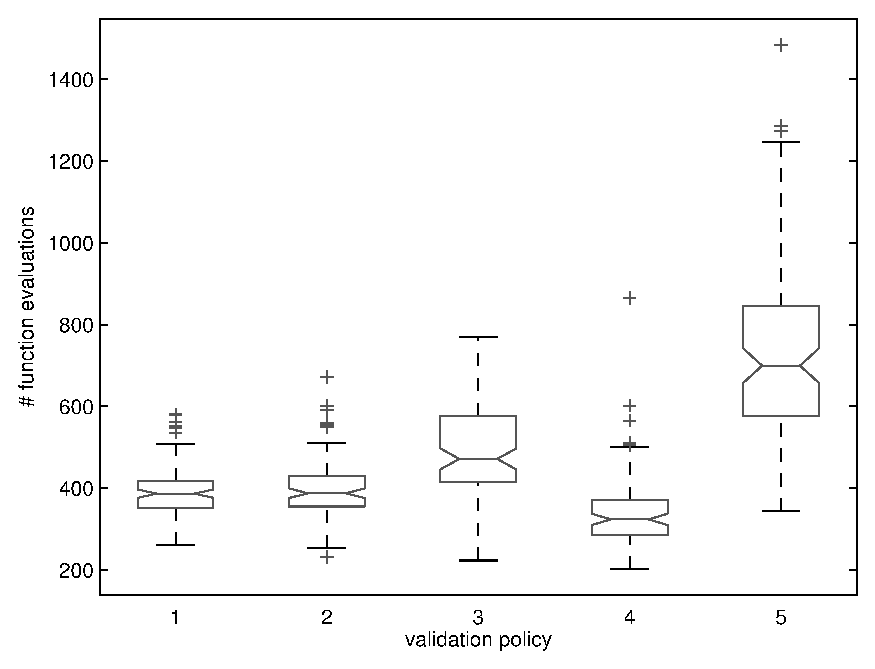
\includegraphics[width=\textwidth]{anova}
\caption[Box plot for different validation strategies]{Box plot for different validation methods~\cref{sur:val:org,sur:val:pseudo,sur:val:first,sur:val:last,sur:val:mubest} for Rosenbrock function of dimension $d=2$.}
\label{fig:boxplot}
\end{figure}

The surrogate ranking validation and improvement strategy using ordinal regression is tested using a Covariance Matrix Adaptation Evolution Strategy (CMA-ES) developed by \cite{Hansen01}. CMA-ES is a very efficient numerical optimization technique, however we still expect to reduce the number of function evaluations needed for search. For \cite{Ru06:PPSN} the validation policy had to successfully rank all of the candidate individuals, i.e.,  until $\tau=1$. %<viðbót vegna rýnis>
If there is no limit to training size then updating the surrogate becomes too computationally expensive, hence the training size needs to be pruned to size to $\overline{l}$. %</viðbót vegna rýnis>
\citeauthor{Ru06:PPSN} reduces the set to a size $\overline{l} = \lambda$ by omitting the oldest individuals first. These are quite stringent restrictions which can be improved upon. 
% Pruning away the worst - instead of the oldest 
The pruning only considers the age of the individuals, however older individuals might still be of more interest than newer ones if their fitness ranks higher. A more sophisticated way of pruning would be omitting the lowest ranking individuals first. 
% Validating on a mean pseudo individual  
Moreover, candidate individuals are generated randomly using a normal distribution, thus a pseudo individual representing their mean could be of interest as an indicator for the entire population, e.g., by validating this pseudo individual first could give information if the surrogate is outdated w.r.t. the current search space. 
% Validation only the current mu best ranked individuals 
Furthermore, the validation is only done on the candidate individuals for the current generation in ES where only the $\mu$ best ranked individuals will survive to become parents. In evolutionary computing one is interested in the accurate ranking of individuals  generated in the neighbourhood of parent individuals, hence for sufficient validation of the surrogate, only the $\mu$ best ranked individuals  should be considered and evaluated, since all other individuals  of lower rank will be disregarded in the next iteration in ES. 
% Validating on every other generation
Lastly, one should also investigate the frequency by which the model is validated, e.g., at each generation or every $K>1$ generations or even have the need for validating adapt with time.

Preliminary tests were conducted on which validation method deemed fruitful, by implementing  Rosenbrock function of dimension $d=2$, for the following setups, 
\begin{inparaenum}[{Method} (i)]
 \item the setup presented in \cite{Ru06:PPSN} %\label{sur:val:org}
 \item omitting the worst individuals during the pruning process, instead of the oldest ones; \label{sur:val:first}
 \item initialise the validation process by using a pseudo individual that represents the mean of the new candidate individuals; \label{sur:val:pseudo}
 \item requiring that only the $\mu$ best candidate individuals are correctly ranked; \label{sur:val:mubest}
\item validating on every other generation. \label{sur:val:last}
\end{inparaenum}
To summarise, the original method~\cref{sur:val:org} is compared with the aforementioned validation improvements, namely methods~\cref{sur:val:first,sur:val:pseudo,sur:val:mubest,sur:val:last}, which were added one at a time to the original method. 


Experimental results focusing on the number of true function evaluations are shown in~\cref{fig:boxplot}. There is no statistical difference between omitting oldest or worst ranked individuals  from the training set, but this was expected, since both are believed to be representatives of a region of the search space which is no longer of interest. Adding the pseudo mean candidate individual didn't increase the performance edge. When the surrogate was updated on every other generation, it quickly became outdated and more than double function evaluations were needed to achieve the same rate of convergence. 
However, requiring the correct ranking for only the $\mu$ best ranked candidate individuals showed a significant performance edge. 

If the training accuracy is not 100\% then clearly $\tau < 1$. In this case additional training individuals  would be forced for evaluation. However, enforcing a completely concordant ranking, i.e.,  $\tau=1$, was deemed to be too strict due to the fact the search is stochastic. Thus the surrogate is said to be sufficiently accurate if $\tau>0.999$. \todo{Af hverju 0.999? Rökstyðja betur}

Based on these preliminary tests, a pseudo code for the proposed model validation and improvement strategy is described in~\cref{fig:pseudocode} where it is implemented at the end of each generation of CMA-ES. The algorithm essentially only evaluates the expensive true fitness function when the surrogate is believed to have diverged. During each iteration of the validation process there are two sets of individuals, $\mathcal{Y}$ and $\mathcal{X}$, which are the training individuals  which have been evaluated with the expensive model, and the candidate individuals (of unknown fitness) for the next iteration of CMA-ES, respectively. The test individuals  of interest are those who are believed to become parent individuals  in the next generation of CMA-ES, i.e.,  the $\mu$ best ranked candidate individuals according to the surrogate $h$. The method uses only a simple cross-validation on a single test individual, the one which the surrogate ranks the highest and has not yet been added to the training set. Creating more test individuals  would be too costly, but plausible. Once a test individual has been evaluated it is added to the training set and the surrogate $h$ is updated w.r.t. $\mathcal{Y}$, cf.~\cref{fig:schema}. This is repeated until the surrogate is said to be sufficiently accurate, which occurs if either,
\begin{description}
  \item[$\tau$ sufficiently close], i.e.,  Kendall's $\tau$ statistic between the ranking of the training set using the surrogate, $\bar{R}$, and its true ranking, $R$, is higher than $0.999$, or 
  \item[$\mu$ best ranked] candidate individuals w.r.t. the current surrogate have been added to the training set.
\end{description}
Note that during each update of the surrogate of the ranking of the $\mu$ best candidate individuals can change. Thus it is possible to evaluate more then $\mu$ test individuals  during each validation iteration. 

Once the validation algorithm has completed, the training set is pruned to a size $\bar{l}=\lambda$ by omitting the lowest ranking individuals . \todo{Af hverju þetta gildi á $\bar{l}$?}

\begin{figure}
\noindent{\footnotesize\begin{tabbing}
\quad \quad \= 0\;\; \= \emph{Initialization}: Let $\mathcal{Y}$ denote current training set and its \\
\>   \> corresponding surrogate by $h$. Let $\mathcal{X}$ denote population \\
\>   \> of $\lambda$ individuals of unknown fitness under inspection.\\
\>1  \> {\bf for} \= $t := 1$ to $\lambda$ {\bf do} \emph{(validate a test individual )}\\ 
\>2  \>\> Estimate ranking of $\mathcal{X}$ using $h$; denoted by $\bar{R}_0$. \\
\>3  \>\> $\vec{x}_B \leftarrow \max_{\vec{x}\in\mathcal{X}\setminus\mathcal{Y}}\left\{\bar{R}_0\right\}$ (\emph{test individual}). \\
\>4  \>\> Rank $\vec{x}_B$ w.r.t. individuals  in $\mathcal{Y}$ using $h$; denoted by $\bar{R}$. \\
\>5  \>\> Evaluate $\vec{x}_B$ using true fitness function and evaluate its\\
\>   \>\> true rank among individuals  in $\mathcal{Y}$; denoted by $R$. \\ 
% In the case where no explicit fitness function can be defined, the test individual is evaluated by comparing it with selected individuals  in the training set.
\>6  \>\> $\mathcal{Y}\leftarrow\mathcal{Y}\cup\{\vec{x}_B\}$ \emph{(add to training set)}. \\
\>7  \>\> Compare the rankings  $\bar{R}$ and $R$ by computing the rank \\
\>   \>\> correlation $\tau$.\\
\>8  \>\> {\bf if} \= $\tau>0.999$ {\bf then} \\
\>9  \>\> \> break (\emph{model is sufficiently accurate}) \\
\>10 \>\> {\bf fi} \\
%This is a simple cross-validation on a single test individual. Creating more test individuals  would be too costly, but plausible.
\>11  \>\> Update the surrogate $h$ using the new training set $\mathcal{Y}$.\\
\>12  \>\> {\bf if} \= $\mu$ best individuals of $\bar{R}_0$ have been evaluated {\bf then} \\
\>13  \>\> \> break (\emph{model is sufficiently accurate}). \\
\>14  \>\> {\bf fi} \\
\>15  \> {\bf od} %  Repeated the steps 1-9 above until $\tau_t>0.999$ or at least the $\mu$  highest ranking individuals  of unknown fitness have been evaluated. There is no need to evaluate more than the $\mu$ best ranking individuals  since they will be disregarded in the next iteration of CMA-ES.
\end{tabbing}}
\caption{Pseudo code}
\label{fig:schema:pseudocode}
\end{figure}

\begin{figure} \centering 
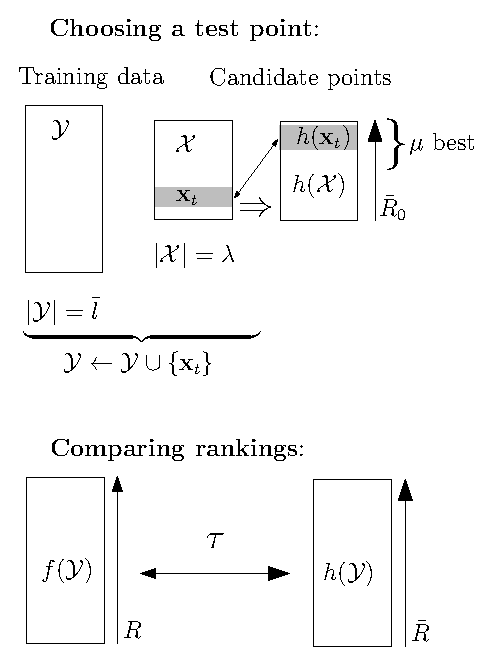
\includegraphics[width=0.5\textwidth]{schema}
\caption{Schema for validating and improving surrogate models.}\label{fig:schema} 
\end{figure}


\section{Experimental Study}\label{sec:sur:expr}
In the experimental study CMA-ES  is run for several test functions, namely sphere model and Rosenbrock function (cf.~\cref{app:fun:sphere} and~\cref{app:fun:rosen}), of various dimensions $d=2,5,10$ and $20$. The average fitness for $100$ independent runs versus the number of function evaluations is reported using the original validation procedure presented in \cite{Ru06:PPSN} and compared with its new and improved validation procedure, whose pseudo code is presented in~\cref{fig:schema:pseudocode} and shown schematically in~\cref{fig:schema}. The procedures will be referred to as using ``all'' or only the ``$\mu$ best'' candidate individuals during the validation, respectively.
The parameter setting for the $(\mu,\lambda)$ CMA-ES is as recommended in \cite{Hansen01} with population size $\lambda = 4+\lfloor 3\ln(n)\rfloor$ and the number of parents selected $\mu=\lambda/4$. The stopping criteria used are $1000n$ function evaluation or a fitness less than $10^{-10}$. The initial mean search individual is generated from a uniform distribution between $0$ and $1$. It is also noted that the training set is only pruned to size $\overline{l} = \lambda$ subsequent to the validation and improvement procedure.

\subsection{Sphere model}\label{sec:sphere}
The first experimental results are presented for the unimodal sphere model of dimension $d$.  
The average fitness versus the number of function evaluations is presented in~\cref{fig:sphereFitness}. A performance edge is achieved by restricting the validation strategy to only having the surrogate correctly rank the $\mu$ highest ranking individuals, and thereby saving the algorithm of evaluating individuals  that would have been disregarded in the next iteration.~\cref{fig:sphereIntmEval} shows the mean intermediate function evaluations that are calculated during the validation process. As one expects, requiring the method to evaluate no more than the $\mu$ best ranked candidate individuals results in a lower intermediate function evaluations, generally saving the method one function evaluation per generation, it also achieves a better mean fitness, as shown in~\cref{tbl:Sphere}.

\begin{figure}
%\subfloat[Mean fitness values versus number of function evaluation]{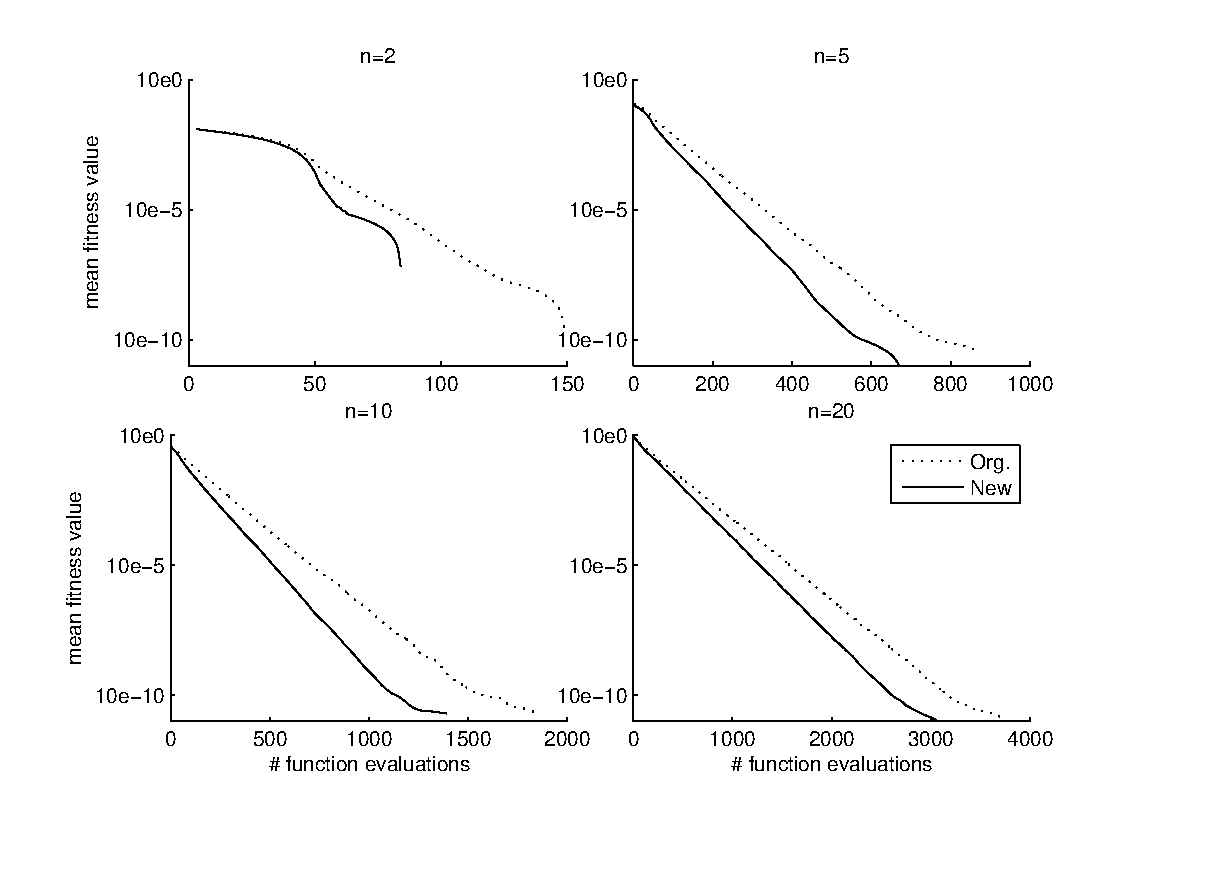
\includegraphics[trim = 8mm 10mm 10mm 5mm, clip, width=\textwidth]{sphere_meanFitness_funcEval}}
\label{fig:sphereFitness}
\,
%\subfloat[Mean intermediate function evaluations versus generation]{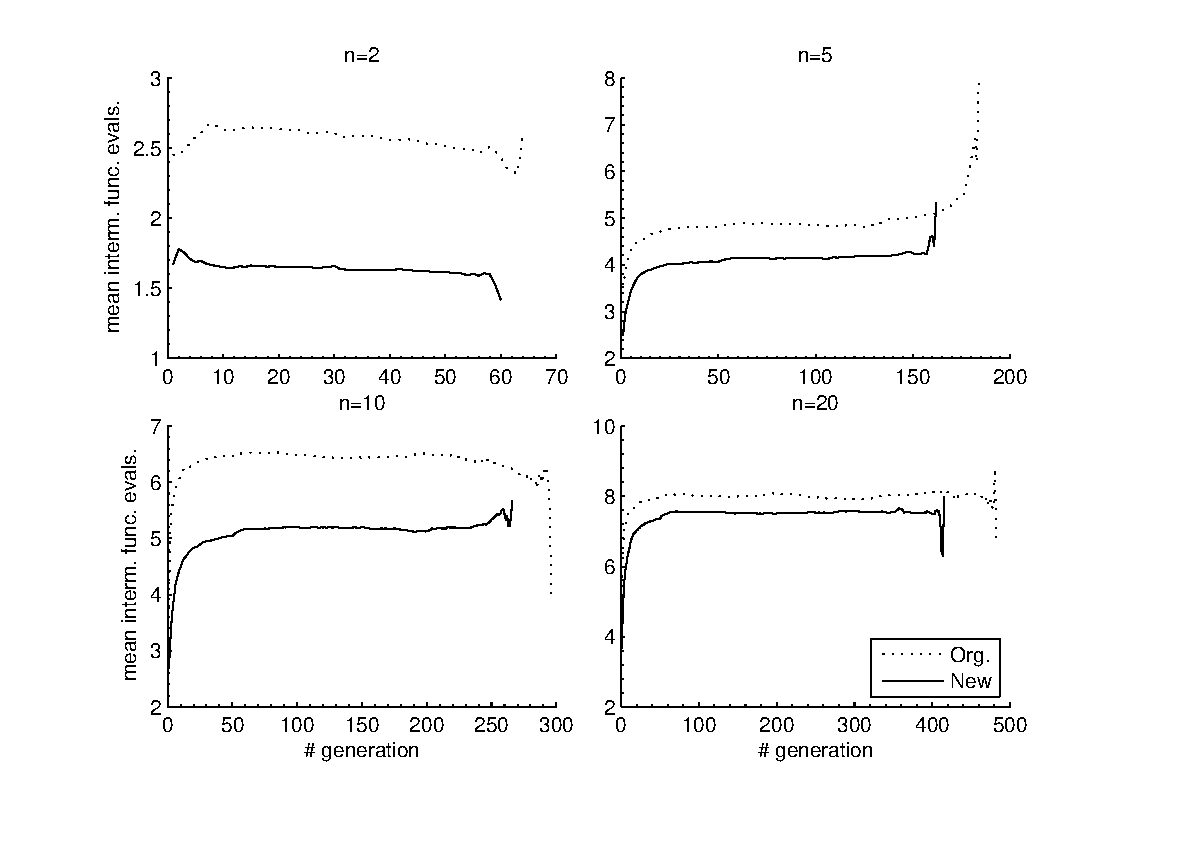
\includegraphics[trim = 10mm 10mm 10mm 5mm, clip, width=\textwidth]{sphere_intmEvals_gen}}
\label{fig:sphereIntmEval}
\caption{Sphere model: Surrogate updated using all (dotted) or $\mu$ best (solid) individuals.}
\end{figure}

\begin{table} \centering
\caption{Main statistics of experimental results for updating surrogate with all or $\mu$ best individuals on sphere model.}\label{tbl:Sphere}
{\renewcommand{\arraystretch}{1.1} \renewcommand{\tabcolsep}{0.1cm} %\scriptsize%footnotesize
\begin{tabular}{ c  c | rrr | rrr| rrr }
\toprule
 & & \multicolumn{3}{c|}{Function eval.} & \multicolumn{3}{c|}{Generations} & \multicolumn{3}{c}{Fitness} \\ 
     & $n$ & \multicolumn{1}{c}{mean} & \multicolumn{1}{c}{med.} & \multicolumn{1}{c|}{sd} & \multicolumn{1}{c}{mean} & \multicolumn{1}{c}{med.} & \multicolumn{1}{c|}{sd} & \multicolumn{1}{c}{mean} & \multicolumn{1}{c}{med.} & \multicolumn{1}{c}{sd} \\
\midrule
all& 2 & 130.59 & 132 & 18.33 & 49.02 & 49 & 6.51 & 2.35e-09 & 2.82e-10 & 1.15e-08\\ 
$\mu$&2 & 81.53 & 81 & 9.53 & 48.11 & 48 & 5.02 & 7.01e-10 & 2.26e-10 & 1.35e-09\\ \midrule
all& 5 & 702.02 & 702 & 67.57 & 145.15 & 145 & 14.96 & 2.77e-10 & 1.82e-10 & 3.64e-10\\ 
$\mu$& 5 & 545.25 & 547 & 54.27 & 132.60 & 132 & 11.03 & 1.83e-10 & 1.46e-10 & 1.09e-10\\ \midrule
all& 10 & 1563.58 & 1553 & 117.09 & 241.83 & 240 & 18.47 & 1.52e-10 & 1.37e-10 & 5.03e-11\\ 
$\mu$& 10 & 1161.03 & 1158 & 79.98 & 226.60 & 224 & 13.86 & 1.34e-10 & 1.22e-10 & 3.80e-11\\ \midrule
all& 20 & 3383.83 & 3377 & 135.52 & 423.14 & 424 & 20.42 & 1.27e-10 & 1.21e-10 & 2.51e-11\\ 
$\mu$& 20 & 2795.28 & 2804 & 132.77 & 372.86 & 372 & 16.56 & 1.17e-10 & 1.12e-10 & 1.72e-11\\ 
\bottomrule
\end{tabular}
}
\end{table}

\subsection{Rosenbrock function}\label{sec:rosen}
The first experiment is now repeated for Rosenbrock function.
The average fitness versus the number of function evaluations is presented in~\cref{fig:rosenFitness} and~\cref{fig:rosenIntmEval} shows the mean intermediate function evaluations that are calculated during the validation process. Despite requiring more generations, the over all function evaluations are significantly lower and yield a better fitness when updating the surrogate on only the $\mu$ best individuals as shown in~\cref{tbl:Rosenbrock}. If all of the candidate individuals have to be ranked correctly, the method will get stuck in local minima for this problem in around 6 out of 100 experiments, however this is not a problem if only the $\mu$ best candidate individuals are ranked consistently, except at high dimensions, and even then the $\mu$ best individuals  policy significantly outperforms evaluating all of the candidate individuals. Clearly the choice of validation policy will influence search performance. 

\begin{figure}
%\subfloat[Mean fitness values versus number of function evaluation]{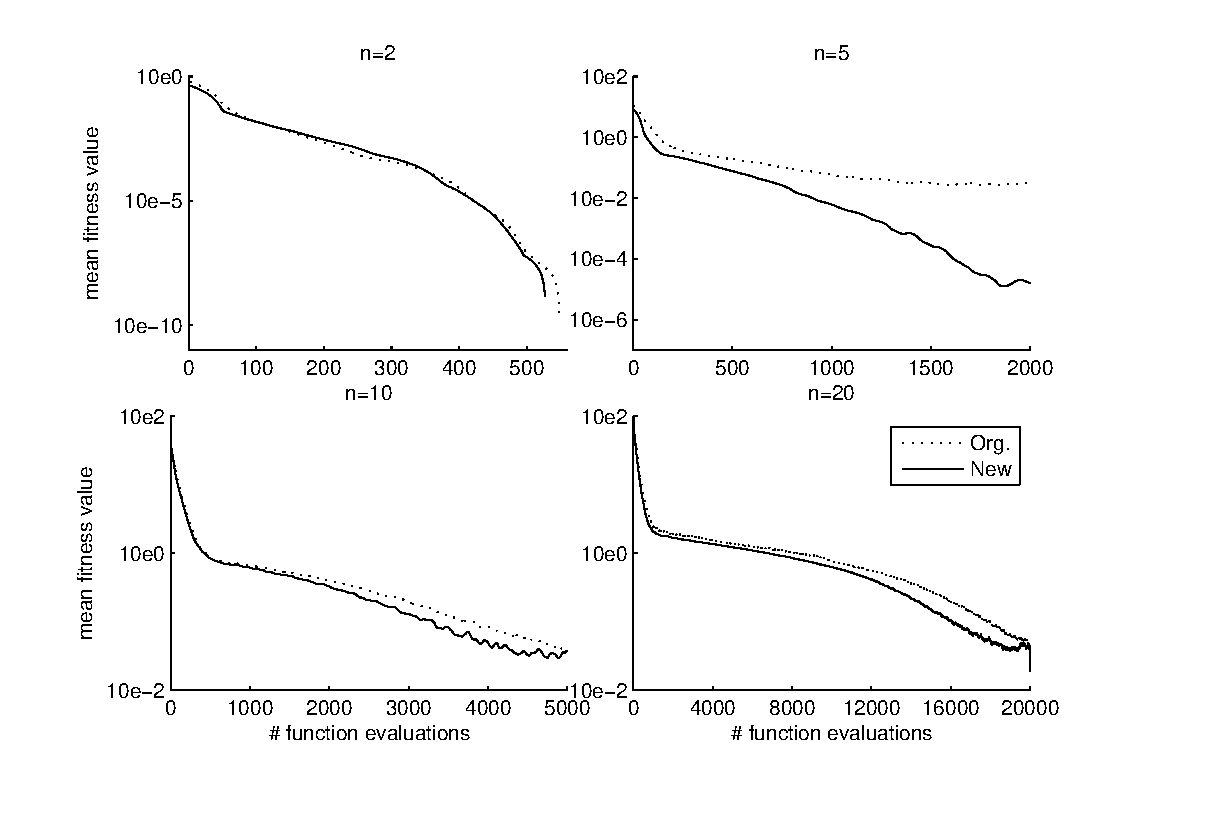
\includegraphics[trim = 10mm 10mm 10mm 5mm, clip, width=\textwidth]{rosen_meanFitness_funcEval}}
\label{fig:rosenFitness}
\,
%\subfloat[Mean intermediate function evaluations versus generation]{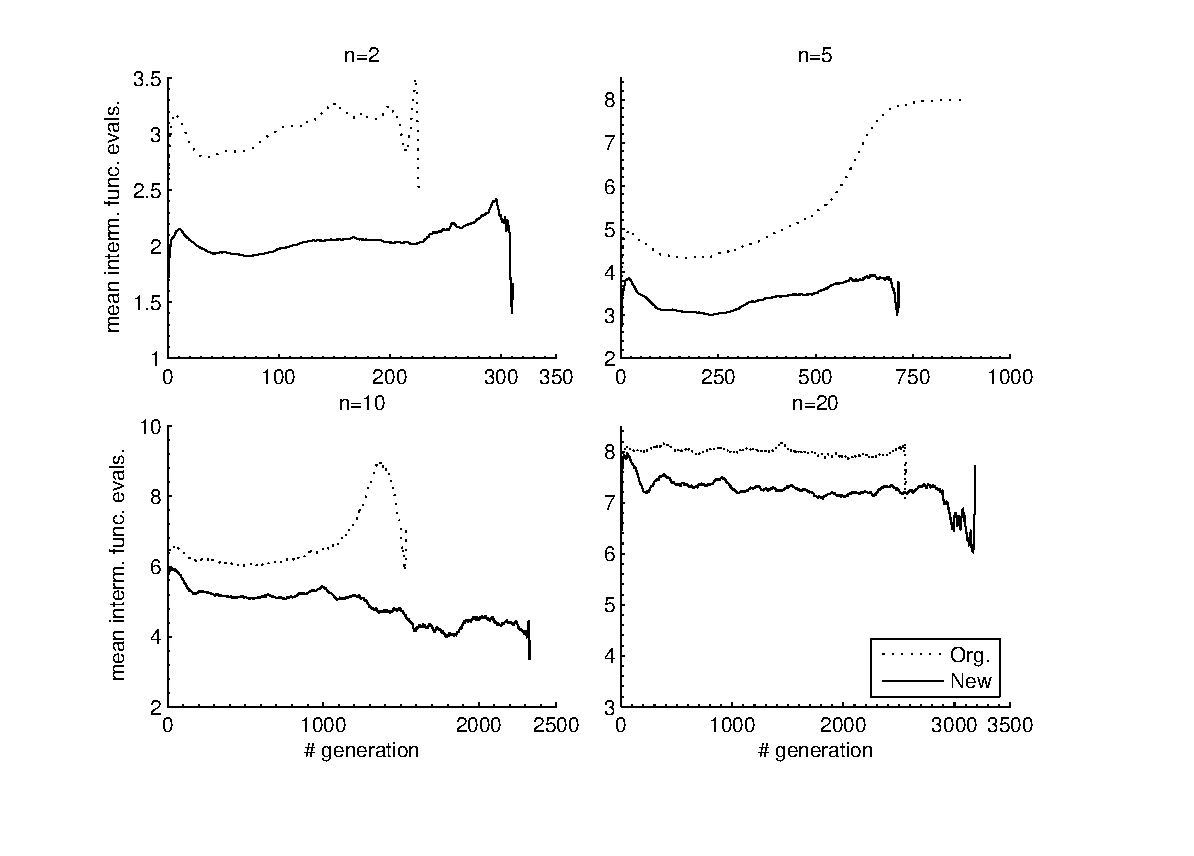
\includegraphics[trim = 15mm 10mm 15mm 5mm, clip, width=\textwidth]{rosen_intmEvals_gen}}
\label{fig:rosenIntmEval}
\caption{Rosenbrock function: Surrogate updated using all (dotted) or $\mu$ best (solid) individuals.}
\end{figure}

\begin{table}\centering
\caption{Main statistics of experimental results for updating surrogate with all or $\mu$ best individuals on Rosenbrock function.} \label{tbl:Rosenbrock}
{\renewcommand{\arraystretch}{1.1} \renewcommand{\tabcolsep}{0.1cm} %\scriptsize%footnotesize
\begin{tabular}{ c  c | rrr | rrr| rrr}
\toprule
 & & \multicolumn{3}{c|}{Function eval.} & \multicolumn{3}{c|}{Generations} & \multicolumn{3}{c}{Fitness} \\ 
     & $n$ & \multicolumn{1}{c}{mean} & \multicolumn{1}{c}{med.} & \multicolumn{1}{c|}{sd} & \multicolumn{1}{c}{mean} & \multicolumn{1}{c}{med.} & \multicolumn{1}{c|}{sd} & \multicolumn{1}{c}{mean} & \multicolumn{1}{c}{med.} & \multicolumn{1}{c}{sd} \\
\midrule
all & 2 & 389.9 & 386 & 63.9 & 132.3 & 130 & 31.3 & 6.24e-10 & 3.20e-10 & 1.05e-09\\ 
$\mu$ & 2 & 344.9 & 336 & 78.6 & 172.2 & 170 & 50.0 & 7.53e-10 & 1.66e-10 & 3.64e-09\\ \midrule
all & 5 & 2464.2 & 2280 & 748.6 & 514.6 & 492 & 105.8 & 2.75e-01 & 1.74e-10 & 1.01e+00\\ 
$\mu$ & 5 & 1724.9 & 1729 & 295.6 & 520.7 & 520 & 82.8 & 1.83e-10 & 1.53e-10 & 1.05e-10\\ \midrule
all & 10 & 6800.5 & 6495 & 1258.7 & 1079.8 & 1052 & 177.8 & 2.79e-01 & 1.32e-10 & 1.02e+00\\ 
$\mu$ & 10 & 6138.5 & 6143 & 1398.2 & 1177.7 & 1103 & 310.1 & 1.99e-01 & 1.24e-10 & 8.73e-01\\ \midrule
all & 20 & 19968.8 & 20004 & 234.7 & 2494.0 & 2500 & 49.6 & 4.54e-01 & 2.88e-02 & 1.08e+00\\ 
$\mu$ & 20 & 19645.9 & 20002 & 1086.4 & 2687.3 & 2748 & 230.5 & 3.10e-01 & 3.12e-07 & 9.97e-01\\ \bottomrule
\end{tabular}
}

\end{table}

\section{Discussion and Conclusion}\label{sec:sur:disc}
The technique presented in this dissertation to control the number of true fitness evaluations is based on a single test individual chosen from a set of candidate individuals which the surrogate ranks the highest. The approximate ranking of this test individual is compared with its true ranking in order to determine the quality of the surrogate. This is a simple form of cross-validation. An alternative approach could be to rank all candidate individuals along with the training individuals  using the surrogate model. This is followed by the re-ranking of training and candidate individuals using the updated surrogate and comparing it with the previous estimate by computing Kendall's $\tau$. Its aim is to observe a change in ranking between successive updates of the surrogate. This study has shown that during the validation process it is sufficient for $\tau$ to be close to $1$ or that only the potential parent individuals should be ranked consistently. \todo{Report \% close to 1 vs. only $\mu$ best}.\\
Moreover, the new validation approach reduces the number of fitness evaluation needed, without a loss in performance although it might take a few more iterations in CMA-ES. 


When it comes to modelling surrogates based on training data, the general rule of thumb is the bigger the training set, the more accurate a model. However, there are computational time limits thus pruning of the training set is necessary. Previous studies \citep{Jin05,Ratle99} have reported that replacing random training individuals  is not optimal. This study has shown that there is no statistical difference in omitting oldest or lowest-ranking individuals  from the training set. Hence, for future work, further investigation on the fitness landscape is needed to determine effectively which search area is no longer of interest and thus unnecessary for the surrogate to approximate correctly. For instance it could be of interest to disregard training individuals  with the largest euclidean distance away from the current candidate individuals rather than simply omitting the oldest/lowest-ranking training individuals. 

When building surrogates in evolutionary computation one is interested in the quality of ranking of individuals  rather than their exact fitness value. For this reason the training accuracy and cross validation is a more meaningful measure of quality for the surrogate model. This is in contrast to regression, where the fitness function is modelled directly and the quality estimated in terms of measures such a least square error. 
This study has shown that the sampling used for validating the accuracy of the surrogate can stop once the $\mu$ best ranked candidate individuals have been evaluated, since they are the only candidate individuals who will survive to become parents in the next generation. 
Although in some cases the sampling could stop sooner, when the surrogate ranking and true ranking are sufficiently concordant, i.e.,  $\tau$ was close to 1. This slight slack in for $\tau$ is allowed due to the fact the ES search is stochastic, however the allowable range in slack for $\tau$ needs to be investigated more fully % <viðbót vegna rýnis>
since allowing only $\tau\in[0.999,1]$ might be too narrow an interval, resulting in an excess of expensive function evaluations needed. %</viðbót vegna rýnis>

However, in the context of surrogate-assisted optimization the discrepancy between the exact model and its surrogate can be translated as noise, which could be an indicator of the necessary sampling size for validation/updating the surrogate, instead of only focusing on consistently ranking the $\mu$ best candidate individuals. Therefore, one can take inspiration from a varying random walk population model suggested by \cite{Miller97} to approximate the population sizing to overcome unnecessary fitness evaluations.
